\begin{frame}[ctb!]
\frametitle{Cyder Advective Diffusive Sensitivity}
Increased advection and increased diffusion lead to greater release. Also, when both are varied, a boundary between diffusive and advective
regimes can be seen. An example of these results are shown in Figure 
\ref{fig:dr_adv_diff}.
\begin{figure}[ht]
\centering
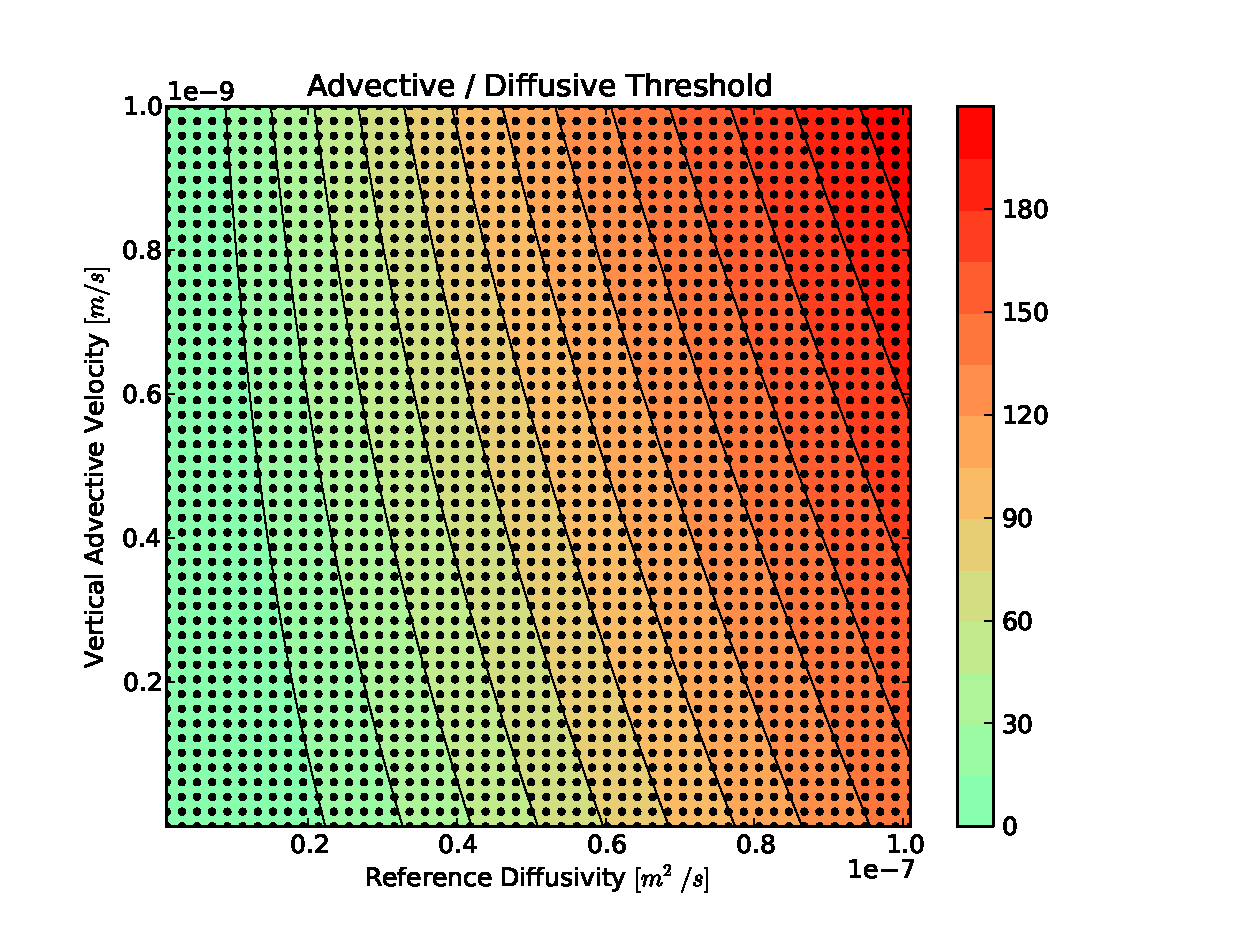
\includegraphics[width=\linewidth]{./nuclide_demonstration/adv_vel_diff.eps}
\caption[Advection vs. Diffusion Sensitivity in Cyder]{Dual advective velocity 
and reference diffusivity sensitivity for a non-sorbing, infinitely soluble 
nuclide.}
\label{fig:dr_adv_diff}
\end{figure}
\end{frame}
